% Drawing 154/01-14 -- folder 154, batch 01, archive page 20 (PDF page 21).
% Transcription: page sans texte : seulement, en haut, un dessin en couleurs sur la même situation que page 19 --- quelques pseudo-droites orange dont trois concourent en un point marqué, une droite jaune $D$ en dessous, la spécialisation en pointillé jaune qui monte vers ce point, et des traits bleus (pleins et pointillés) parallèles à $D$ de part et d'autre du sommet
% Kind: pseudolines with three concurrent at a vertex, line D and its specialisation. Method 2 (schematic redraw from the facsimile). Status: ok.
% Notes: Six orange pseudolines, three of them concurrent at a marked point; the yellow line D below, its specialisation dotted in yellow rising to that point; short blue strokes, solid and dotted, parallel to D above and below the vertex and on D. Drawn over the printed computer listing (upside down), which is not reproduced. D is not labelled on the facsimile.
% Coordinates: 1 unit = 1 mm = 1/100 of the crop width (bbox in page fractions: [0.365, 0.095, 0.551, 0.22]).
% Redrawn by Claude (claude-opus-5-5), issue #73, 2026-11-07; not checked by a human; not compiled (no TeX in the session).
% Revised by Claude (claude-opus-5-5) 2026-11-09 (issue #128) after Michel's check: vertices snapped to exact intersections (drawn points on their lines, meeting ends on the stroke they meet, near-concurrent lines through one computed point, curve ends on their rim); labels at \small as in folder 80 batch 3. Status: ok.
% Rights: reproduces part of the work -- behind RENDER_TRANSCRIPTS, never published by itself.
\documentclass[tikz,border=3pt]{standalone}
\usepackage{amsmath,amssymb}
\usetikzlibrary{patterns,arrows.meta}
\tikzset{Or/.style={orange!90!black}, Ye/.style={yellow!80!orange}, Lg/.style={green!60!black!70}, Dg/.style={green!45!black}, Br/.style={brown!80!black}, Rd/.style={red!85!black}, Bl/.style={blue!70!black}, Gy/.style={black!40}, pencil/.style={black!45}, struck/.style={black!35}, mark/.style={circle,draw,inner sep=1.3pt}, pt/.style={circle,fill,inner sep=0.9pt}, opt/.style={circle,draw,fill=white,inner sep=1.1pt}}
\begin{document}
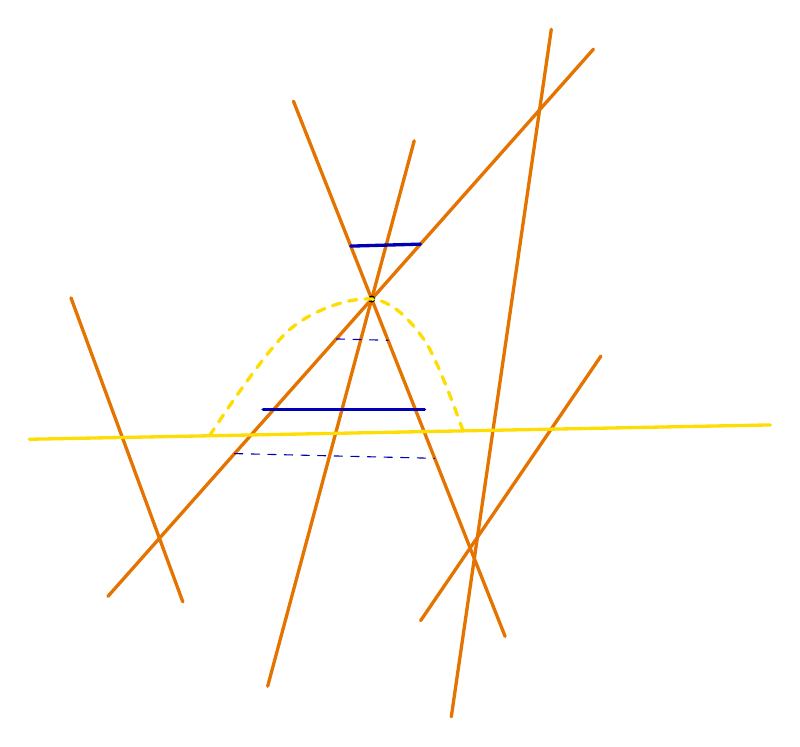
\begin{tikzpicture}[x=1mm,y=1mm,line cap=round,line join=round,font=\scriptsize]
\draw[Or,very thick] (35.55,-13.02) -- (62.43,-80.99);
\draw[Or,very thick] (50.89,-18.05) -- (32.28,-87.32);
\draw[Or,very thick] (73.66,-6.41) -- (11.99,-75.91);
\draw[Or,very thick] (68.3,-3.9) -- (55.6,-91.2);
\draw[Or,very thick] (7.3,-38) -- (21.5,-76.6);
\draw[Or,very thick] (74.6,-45.4) -- (51.7,-79);
\node[pt] at (45.49,-38.15) {};
\draw[Ye,very thick] (2.01,-55.96) -- (96.11,-54.14);
\draw[Ye,dashed,very thick] plot[smooth, tension=0.55] coordinates {(24.9,-55.51) (35.1,-42) (45.49,-38.15) (52.2,-43.4) (57.09,-54.89)};
\draw[Bl,very thick] (42.83,-31.43) -- (51.68,-31.18);
\draw[Bl,dashed] (41,-43.22) -- (47.56,-43.39);
\draw[Bl,very thick] (31.7,-52.2) -- (52.2,-52.2);
\draw[Bl,dashed] (28.08,-57.78) -- (53.49,-58.38);
\end{tikzpicture}
\end{document}
